% A rectangle (step) function on [a,b] with breakpoints t_0,...,t_4:
% left-closed, right-open constant pieces.
% Source: book/tex/calculus/integrate.tex (§ Defining the Riemann integral).
\documentclass[border=2mm]{standalone}
\usepackage{tikz}
\begin{document}
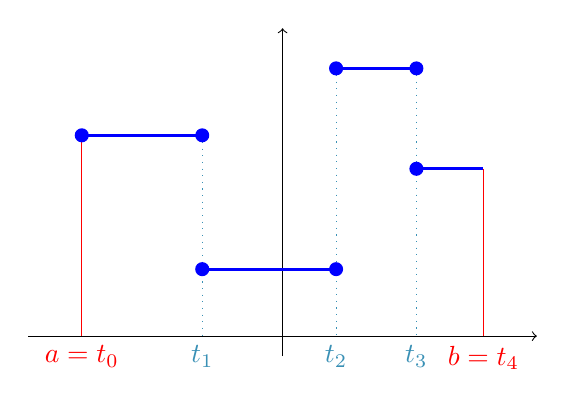
\begin{tikzpicture}[scale=0.85,
    dot/.style={circle,fill,inner sep=1.8pt},
    odot/.style={circle,draw,fill=white,inner sep=1.5pt,thick}]
  \draw[->] (-3.8,0)--(3.8,0);
  \draw[->] (0,-0.3)--(0,4.6);
  % constant pieces (blue)
  \draw[blue,line width=1.2pt] (-3,3)--(-1.2,3);
  \draw[blue,line width=1.2pt] (-1.2,1)--(0.8,1);
  \draw[blue,line width=1.2pt] (0.8,4)--(2,4);
  \draw[blue,line width=1.2pt] (2,2.5)--(3,2.5);
  % boundary verticals
  \draw[red] (-3,3)--(-3,0);
  \draw[red] (3,2.5)--(3,0);
  \draw[cyan!70!black,dotted] (-1.2,3)--(-1.2,0);
  \draw[cyan!70!black,dotted] (0.8,4)--(0.8,0);
  \draw[cyan!70!black,dotted] (2,4)--(2,0);
  \node[red,below] at (-3,0) {$a=t_0$};
  \node[red,below] at (3,0) {$b=t_4$};
  \node[cyan!70!black,below] at (-1.2,0) {$t_1$};
  \node[cyan!70!black,below] at (0.8,0) {$t_2$};
  \node[cyan!70!black,below] at (2,0) {$t_3$};
  % endpoint dots: closed on the left of each step, open on the right
  \node[dot,blue] at (-3,3) {};
  \node[dot,blue] at (-1.2,1) {};
  \node[dot,blue] at (0.8,4) {};
  \node[dot,blue] at (2,2.5) {};
  \node[odot,blue] at (-1.2,3) {};
  \node[odot,blue] at (0.8,1) {};
  \node[odot,blue] at (2,4) {};
\end{tikzpicture}
\end{document}
